\chapter[THEORETICAL FRAMEWORK]{\huge THEORETICAL FRAMEWORK}
In this chapter are mentioned some concepts behind the methods used in this work. In the first section are boarded some generalities of EEG signals, which include a description of their generation, mental activities associated with sub-bands, and conventional data acquisition techniques. The next section encompasses introductory concepts of wavelet functions and their usage for EEG data. Later in another section, two neuron models are briefly described, which were implemented in some classifiers used in this work. At the end of this chapter, the generalities of these classifiers are also explained.\\

\section{Electroencephalography}
The electroencephalography was used in humans for the first time in 1924 by the psychiatrist Hans Berger, who suggested that periodicities in EEG signals may be associated with mental activities. Later on, at the end of the last century, many technologies were developed and enhanced to record brain activity, which includes fMRI, PET, MEG, EEG, and NIRS.\\

In the case of EEG, a good time resolution can be achieved with current technologies. Nevertheless, its spatial resolution is limited by the number of channels used, even though a single electrode of $\sim$10 millimeters covers approximately 250000 neurons \cite{pizzagalli2007electroencephalography}. Also, it is assumed that tens of thousands of synchronously activated pyramidal neurons, perpendicular to the cortical surface, generate EEG oscillations. Thus, these oscillations represent the sum of excitatory (positive) and inhibitory (negative) pyramidal neuron's PSPs transmitted among the neural network (a brief description of these process is mentioned in the neuron model's section).\\

Figure \ref{Fig: EEG_Generation} depicts these EEG generation process through three different images. Image \textbf{A.} shows a coronal slice of the human brain. Then, the image \textbf{B.} depicts a zoom in the inset from \textbf{A.}, in which the scalp, skull, and cerebral spinal fluid are represented. Finally, the image \textbf{C.} shows a cortical pyramidal neuron's scheme localized in the inset from \textbf{B.} and from which the closed loops represent the extracellular current's summation.\\

\begin{figure}[h!]
	\centering
	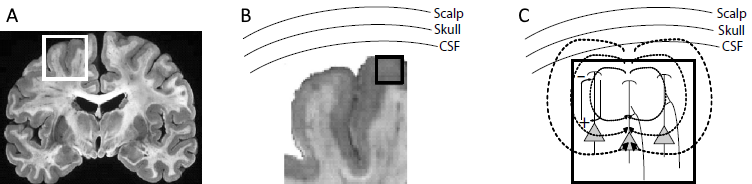
\includegraphics[width=\linewidth]{Figures/EEG_Generation.png}
	\caption{Neurophysiological basis of EEG generation (Figure obtained from \cite{pizzagalli2007electroencephalography}).}
	\label{Fig: EEG_Generation}
\end{figure}

Figure \ref{Fig: EEG_Generation} depicts not only the EEG generation but also the challenges of acquiring these signals due to the different layers between the brain cortex and electrodes, which inevitably distorts the signals. Due to that, a uniform and homogeneous electrode's coverage on the scalp is imperative to avoid additional signal distortions. It is mentioned in \cite{pizzagalli2007electroencephalography} that electrode's distances of 2-3 cm are required to prevent distortions of the potential scalp distribution.\\

Due to this issue, some electrodes placement systems have been proposed, from which the International 10-20 system highlights and consists of placing the electrodes at sites 10\% or 20\% from the total front-back (nasion-inion) or right-left distance of the skull. Furthermore, it is also mentioned in \cite{pizzagalli2007electroencephalography} that several studies suggest at least 60 equally distributed electrodes (or channels) are required for an accurate spatial sampling of scalp activities.\\

Moreover, an EEG signal acquired from a particular channel represents the differential potential between that electrode and a recording reference, which ideally should be electrically inactive. Unfortunately, the reference contributes to recordings, and in some circumstances, it could be contaminated by non-encephalic activity such as muscle or electromyographic artifacts. The particular cases of artifacts caused by blinks and eye movements can be detected and corrected with additional channels that record vertical and horizontal eye movements.\\

According to \cite{pizzagalli2007electroencephalography}, the reference choice is irrelevant for any source location; however, this is not the case for this work due to the lack of overt and imagined speech dynamics knowledge. Nonetheless, several methods have been invented for reference-dependency issues, from which average reference is commonly used and that consists of re-deriving per timestep the EEG signals against the average value across all electrodes.\\

Other EEG preprocessing method used to deal with these issues is the small Laplacian filter, which was mentioned in the previous chapter and was employed during the data collection in \cite{zhao2015classifying}. This method consists of computing the average potential difference between each electrode and the nearest four electrodes to emphasize the shallow cortical generators.\\

In addition to these challenges, the interactions between thalamic and cortical networks produce rhythmical activities, which are associated with particular functions, and their amplitudes typically range from 10 to 100 microvolts. These mental rhythms with their corresponding frequency band range are described as follows \cite{pizzagalli2007electroencephalography}:
\begin{itemize}
	\item \underline{Delta band ($\delta$, 1-4 Hz)}: These oscillations are associated with sleep in healthy people and neurological pathologies, such as brain lesions and tumors. Also, they are predominant in infants during the first two years.
	\item \underline{Theta band ($\theta$, 4-8 Hz)}: It is prominent during sleeping. However, during wakefulness has been linked to decreased alertness, focussed attention, mental effort, and effective stimulus processing.
	\item \underline{Alpha band ($\alpha$, 8-13 Hz)}: This band presents amplitude differences among individuals, which are diminished by sudden alerting, mental concentration, and eye-opening. Fo this reason, it is associated with visual system functions. Besides, in cognitive tasks, lower-alpha (8-10 Hz) suppression has been associated with stimulus-unspecific and task-unspecific increases in intentional demands. While upper alpha (10-12 Hz) desynchronization has been linked to sensory-semantic information processing, semantic memory performance, and stimulus-specific expectancy.
	\item \underline{Beta band ($\beta$, 13-30 Hz)}: It typically replaces $\alpha$ rhythm during cognitive activity. Due to that, the $\beta$ band has been associated with attention and vigilance states. It is also suggested that $\beta$ increases are present during diffuse arousal and focused attention.
	\item \underline{Gamma band ($\gamma$, 36-44 Hz)}: These oscillations have been related to attention, arousal, object recognition, top-down modulation of sensory process, and perceptual binding (brain's ability to integrate various aspects of a stimulus into a coherent whole).
\end{itemize}

All these oscillatory rhythms have their particular aspects. However, they encompass several mental activities that are difficult to select prior experiments in a computer science fashion. For this reason, a method that provides a decomposition of EEG signals close to the bands mentioned here is described in the next section.
\section{Spectral Analysis}
\section{Neuron Models}
\section{Classifiers}
\subsection{NeuCube}
\subsection{Single Spiking Neuron}
Following the same procedure as in \cite{vazquez2010pattern,vazquez2011training}, the training for the SSN consisted of the following steps:
\begin{enumerate}
	\item An initial population is generated, which is composed of a predefined number of individuals. Hence, each individual is a vector from which each element represents an SSN's parameter. In this step, the parameter values are randomly assigned over a predefined interval.
	\item The spiking neuron parameters are set with each individual's values and fed with the training samples.
	\item Each training sample produced a firing activity in the neuron output, from which the firing rate of each is computed. 
	\item The AFR is calculated with the firing rates per associated class.
	\item The third step is performed with the training and test fold data (in Chapter 5 is explained the data split), and, based on the Manhattan distance between the firing rates and the AFRs, each sample is associated with a particular class (the closest, according to the distance).
	\item The individuals for the next generation are built based on the DEA and a fitness function, which consists of summing training and test fold errors.
	\item The process is repeated from step 2 until the number of declared generations is completed. For all the experiments in this work,  500 generations were used.
	\item The best individual was selected (the one with less number of errors) after the last generation was performed.
\end{enumerate}